\documentclass[11pt]{article}
\usepackage[margin=1in]{geometry}
\usepackage{amsmath,amssymb}
\usepackage{tikz}
\usetikzlibrary{positioning,arrows.meta}
\usepackage{enumitem}

\newcommand{\indep}{{\bot\negthickspace\negthickspace\bot}}

\pagestyle{empty}

\begin{document}

\begin{center}
{\Large \textbf{Statistics 256: Causality}} \\[6pt]
{\large In-class Activity 1: DAGs Part 1}
\end{center}

\vspace{4pt}
\noindent\textbf{Name(s):} \hrulefill

\vspace{16pt}

%%% QUESTION 1 %%%
\noindent\textbf{Question 1: $d$-separation}

\medskip
\noindent Consider the following DAG:

\begin{center}
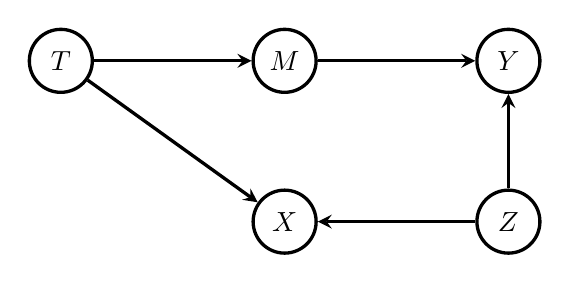
\begin{tikzpicture}[
    ->,>=stealth,
    node distance=2cm,
    every node/.style={circle, draw, minimum size=8mm, inner sep=1pt, font=\normalsize},
    very thick
]
    \node (T) {$T$};
    \node (M) [right=of T] {$M$};
    \node (Y) [right=of M] {$Y$};
    \node (X) [below=1.2cm of M] {$X$};
    \node (Z) [right=of X] {$Z$};

    \draw (T) -- (M);
    \draw (M) -- (Y);
    \draw (T) -- (X);
    \draw (Z) -- (X);
    \draw (Z) -- (Y);
\end{tikzpicture}
\end{center}

\begin{enumerate}[label=(\alph*)]
\item List all paths between $T$ and $Y$ (ignoring arrow direction).

\vspace{1.4cm}

\item Is $T$ $d$-separated from $Y$ given $\emptyset$ (i.e.\ unconditionally)? Explain.

\vspace{1.4cm}

\item Is $T$ $d$-separated from $Y$ given $\{M\}$? Explain.

\vspace{1.4cm}

\item Is $T$ $d$-separated from $Y$ given $\{X\}$? Explain.

\vspace{1.4cm}

\item Is $T$ $d$-separated from $Y$ given $\{M, X\}$? Explain.

\vspace{1.4cm}
\end{enumerate}

%%% QUESTION 2 %%%
\noindent\textbf{Question 2: Draw the DAG}

\medskip
\noindent For each scenario below, draw a DAG that encodes the causal relationships described.  Label every node clearly. You can use a variable "U" for unobserved things you may not have a good name for, though if you can think of something specific, all the better. 

\clearpage

\begin{enumerate}[label=(\alph*)]
\item A researcher wants to know if having more police reduces crime, but the data show that cities with more police actually have more crime. Draw a DAG indicating what might be happening. 

\vspace{3cm}

\item A hiring committee selects candidates based on a combined assessment of interview performance and resum\'e quality.  An analyst examines only the hired candidates and finds that, among them, those with stronger resum\'es appear to have performed worse in interviews. Draw a DAG that explains this pattern. Which node is being conditioned on?

\vspace{3cm}
\end{enumerate}

%%% QUESTION 3 %%%
\noindent\textbf{Question 3: Two researchers, two DAGs}

\medskip
\noindent Two researchers are studying the relationship between exercise ($E$), weight ($W$), and blood pressure ($B$). They agree on the variables but disagree about the causal structure.

\medskip
\noindent \textbf{Researcher 1} believes exercise affects weight, and weight affects blood pressure:

\begin{center}
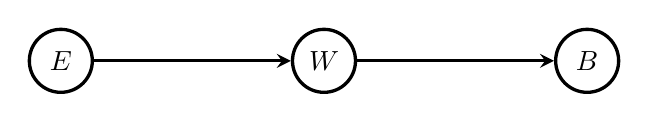
\begin{tikzpicture}[
    ->,>=stealth,
    node distance=2.5cm,
    every node/.style={circle, draw, minimum size=8mm, inner sep=1pt, font=\normalsize},
    very thick
]
    \node (E) {$E$};
    \node (W) [right=of E] {$W$};
    \node (B) [right=of W] {$B$};
    \draw (E) -- (W);
    \draw (W) -- (B);
\end{tikzpicture}
\end{center}

\noindent \textbf{Researcher 2} believes exercise affects both weight and blood pressure directly, and weight also affects blood pressure:

\begin{center}
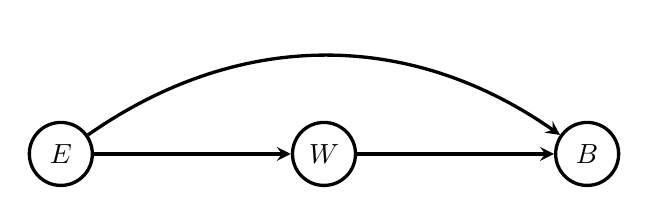
\begin{tikzpicture}[
    ->,>=stealth,
    node distance=2.5cm,
    every node/.style={circle, draw, minimum size=8mm, inner sep=1pt, font=\normalsize},
    very thick
]
    \node (E) {$E$};
    \node (W) [right=of E] {$W$};
    \node (B) [right=of W] {$B$};
    \draw (E) -- (W);
    \draw (W) -- (B);
    \draw (E) to[bend left=35] (B);
\end{tikzpicture}
\end{center}

\begin{enumerate}[label=(\alph*)]
\item Under Researcher~1's DAG, is $E \indep B \mid W$?  Under Researcher~2's DAG, is $E \indep B \mid W$? 

\vspace{1.5cm}

\item Based on your answers, describe a pattern you could look for in data to help distinguish between these two graphs.


\vspace{2.5cm}
\end{enumerate}

%%% QUESTION 4 %%%
%\noindent\textbf{Question 4: From data patterns to DAGs}
%
%\medskip
%\noindent A researcher studying three variables $A$, $B$, and $C$ observes the following in a large dataset:
%
%\begin{itemize}[nosep]
%\item $A$ and $B$ are associated (not independent).
%\item $B$ and $C$ are associated (not independent).
%\item $A$ and $C$ are \textbf{independent} (unconditionally).
%\item $A$ and $C$ are \textbf{not independent} given $B$.
%\end{itemize}
%
%\begin{enumerate}[label=(\alph*)]
%\item Draw a DAG over $\{A, B, C\}$ that is consistent with all four facts above.
%
%\vspace{4cm}
%
%\item Is your DAG the only one consistent with these facts?  If not, draw another DAG that also fits. If so, explain why.
%
%\vspace{4cm}
%
%\item Now suppose the researcher instead found that $A$ and $C$ are \textbf{associated} unconditionally but become \textbf{independent} when conditioning on $B$.  Draw a DAG consistent with this revised pattern. How does the key structure differ from part~(a)?
%
%\vspace{4cm}
%\end{enumerate}
%
\end{document}
